\documentclass[letterpaper]{book}

% Uncomment for bibliog.
%\bibliographystyle{unsrt}

\usepackage{boxedminipage}
\usepackage{graphicx}
\usepackage{fancyhdr}
\usepackage{amsmath}
\usepackage{lineno}
\usepackage{hyperref}
\usepackage{listings}
\usepackage{color}
\usepackage[usenames,dvipsnames,svgnames,table]{xcolor}

% tikz package for block diagrams
\usepackage{tikz}
\usetikzlibrary{arrows,calc,patterns,decorations.pathmorphing,decorations.markings}
\tikzset{>=latex} % blockier style arrow heads


\newcommand{\grad}{\bigtriangledown}
\newcommand{\pd}{\partial}
\newcommand{\br}{\epsilon \mathcal{R}}


%%%%%%%%%%%%%%%%%%%%%%%%%%%%%%%%%%%%%%%%5
%
%  Set Up Margins

%%%%%%%%%%%%%%%%%%%%%%%%%%%%%%%%%%%%%%%%%%%%%%%%%
% include file for:
%      Critical Page setup dimensions
%            DO NOT MODIFY
%       (for help see "Latex Line by Line" p 260)
%
\setlength\oddsidemargin{0in}
\setlength\evensidemargin{0in}

\usepackage[left=0.98in, right=0.98in, top=1.0in, bottom=1.0in]{geometry}

% %Top Margin and header
% \setlength\voffset{-0.94in}
% \setlength\topmargin{0.25in}
% \setlength\headheight{0.25in}
% %\setlength\headwidth{6.5in}
% \setlength\headsep{0.25in}
% %Body
% \setlength\textwidth{6.5in}
% \setlength\textheight{9.50in}
% %Footer
% %\setlength\footheight{0.5in}
% \setlength\footskip{0.3750in}
% Line spacing for 6 lines per inch
\linespread{0.894}  % 1.0 = single    1.6 = double
%
%          END of Critical Page Setup Dimensions
%%%%%%%%%%%%%%%%%%%%%%%%%%%%%%%%%%%%%%%%%%%%%%%%%%%

%%%%%%%%%%%%%%%%%%%%%%%%%%%%%%%%%%%%%%%%%%%%%%%%%%%
%
% Useful style and math macros
%


\newcommand\Dfrac[2]{\frac{\displaystyle #1}{\displaystyle #2}}
\newcommand\beq{\begin{equation}}
    \newcommand\eeq{\end{equation}}

\newcommand\bmat{\begin{bmatrix}}
    \newcommand\emat{\end{bmatrix}}

\newenvironment{solution}
{\ttfamily \vspace{0.155in} {\bf SOLUTION:} \\ }
{ \vspace{0.25in} \par }


% Make table rows deeper
%\renewcommand\arraystretch{2.0}% Vertical Row size, 1.0 is for standard spacing)

% \input{pagedimsmall.tex}

%%%%%%%%%%%%%%%%%%%%%%%%%%%%%%%%%%%%%%%%%%%%%%%%%
%
%         Page format Mods HERE
%
%Mod's to page size for this document
\addtolength\textwidth{0cm}
\addtolength\oddsidemargin{0cm}
\addtolength\headsep{0cm}
\addtolength\textheight{0cm}
%\linespread{0.894}   % 0.894 = 6 lines per inch, 1 = "single'',  1.6 = "double''

%\pagestyle{fancy}
\lhead{Chapter \thechapter}
%\chead{CENTER HEADER}
\rhead{\today}
%\lfoot{Hannaford, U. of Washington}
%\rfoot{\today}
\cfoot{\thepage/\pageref{LastPage}}


%%%%%%%%%%%%%%%%%%%%

%%%%%%%%%%%%%%%%%%%%%%%%%%%%%%%%%%%%%%%%%%%%%%%%%%%%%%
%
%  Example environment
%
\newcounter{Example}[chapter]

\newenvironment{Example}
% begin
{\refstepcounter{Example}\newpage
 \begin{boxedminipage}{\textwidth} % \linenumbers
    {\bf Example \thechapter.\theExample}\\
}
% end
{\vspace{0.1in}\end{boxedminipage}
\vspace{0.4in} }

\newenvironment{ExampleCont}
% begin
{
 \begin{boxedminipage}{\textwidth}\linenumbers
    {\bf Example \thechapter.\theExample \hspace{4pt} cont.}\\
}
% end
{\vspace{0.1in}\end{boxedminipage}
\vspace{0.4in} }


\newenvironment{ExampleSmall}
% begin
{\refstepcounter{Example}
\vspace{0.2in}
 \begin{boxedminipage}{\textwidth}
    {\bf Example \thechapter.\theExample}\\
}
% end
{\vspace{0.05in}\end{boxedminipage}
\vspace{0.25in} }
%
%%%%%%%%%%%%%%%%%%%%%%%%%%%%%%%%%%%%%%%%%%%%%%%%%%%%%


%%%%%%%%%%%%%%%%%%%%%%%%%%%%%%%%%%%%%%%%%%%%%%%%%%%
%
%    Minted package for nice python highlighting
%
\usepackage[chapter]{minted}  % python syntax highlight

% Required packages

% Configure minted styling
\setminted[python]{
    frame=lines,
    framesep=2mm,
    baselinestretch=1.0,
    fontsize=\footnotesize,
    linenos=true,
    breaklines,
    %     style=monokai,
    style=default
}
\setminted[C]{
    frame=lines,
    framesep=2mm,
    baselinestretch=1.0,
    fontsize=\footnotesize,
    linenos=true,
    breaklines,
    %     style=monokai,
    style=default
}

% Configure listing to have a specific width
\setminted{
    numbersep=2pt,    % Distance between line numbers and code
    xleftmargin=20pt, % Left margin (increase if line numbers still overflow)
    xrightmargin=-2pt  % Right margin (decrease to reduce extra white space)
}

% Configure listing caption style
\DeclareCaptionFormat{listing}{\raggedright#1#2#3}
\captionsetup[listing]{
    format=listing,
    labelfont=bf,
    font=small,
    labelsep=period
}

%%%%%%% end of minted %%%%%%%%%%%%%%%%%%%%%%%%%%%%%%%%%%%%%%%%%%%%


%%%%%%%%%%%%%%%%%%%%%%%%%%%%%%%%%%%%%%%%%%%%%%%%%%%%%%%%%%%%%%
%       Claude formatting code begins here
\definecolor{claudeBlue}{RGB}{59, 89, 152}
\definecolor{claudeGray}{RGB}{242, 244, 248}

\newcommand{\humanquery}[1]{%
  \par\vspace{\baselineskip}%
  \noindent%
  \fbox{%
    \parbox{\dimexpr\linewidth-2\fboxsep-2\fboxrule\relax}{#1}%
  }%
  \par\vspace{\baselineskip}%
}

\newcommand{\claudereply}[1]{%
  \par\vspace{\baselineskip}%
  \noindent%
  \fcolorbox{claudeBlue}{claudeGray}{%
    \parbox{\dimexpr\linewidth-2\fboxsep-2\fboxrule\relax}{%
      \ttfamily\raggedright #1%
    }%
  }%
  \par\vspace{\baselineskip}%
}
%%%%%%%%%%%%%%%%%%%%%%%%%%%%%%% Claude formatting code ends here


%
%   quick type equation envir.
%
\def\bq{\begin{equation}}
\def\eq{\end{equation}}

% Symbol defs for equations
\def\ef{\mathcal{E}}
\def\fl{\mathcal{F}}

% Laplace Transform
\newcommand{\sL}{\mathcal{L}}



\begin{document}  

\section{State Space System Representation}
Most of this course will cover control system design using system transfer functions (rational polynomials in $s$ which describe the input-output relationships of system blocks).  However when we write the equations of motion, it is an ideal time to introduce a couple of concepts from the ``modern control theory'' introduced in the 1960's which has supplanted the $s$ domain methods in some applications.  

In ``modern'' control theory, the system is represented as a first order linear differential equation in a high diminsional space known as state space.  Each point in state space represents a unique dynamical state of the system.   For example, a system with one mass could be described by a 2-dimensional state space consisting of the position, $x$ and the velocity, $\dot{x}$ (Figure \ref{2Dstatespace}).

\begin{figure}\centering
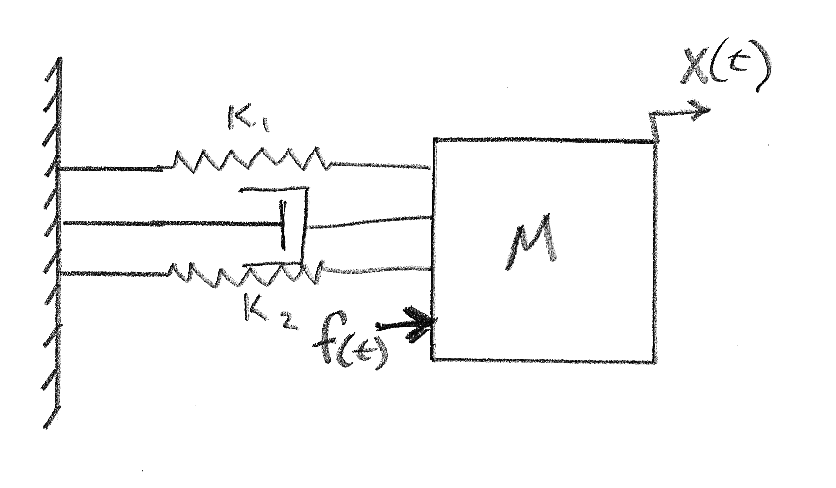
\includegraphics[width=65mm]{figs03/01069.png}
\caption{Translational dynamic system for state space example.}\label{2Dstatespace}
\end{figure}

One way to define the dimensions of state space is to identify all system variables which describe an energy.  Each one is a dimension of state space.   In our single mass example, energy is stored in the spring and mass:
\[
E_K = \frac{1}{2}Kx^2 \qquad E_M = \frac{1}{2}M{\dot{x}}^2
\]

We use a vector, $X$ to define a point in state space such as:
\[
X = \begin{bmatrix} x \\ \dot{x} \end{bmatrix}
\]
Then the dynamics of the system are represented in a matrix first order LODE:
\[
\dot{X} = AX+BU
\]
Where $X$ is the state vector, $\dot{X}$ is the first derivative of the state vector,
$A$ is a matrix of coefficients, $U$ is the system input (like an applied force, $f(t)$, and 
$B$ is another matrix. 

Sometimes the output of the system, $Y$, is not one of the state variables, but instead a linear
combination of the state variables.  In this case there is another equation 
\[
Y = CX+DU
\]
where $C,D$ are additional matrices of coefficients.   There is no Laplace transform and the 
equations come directly from the equations of motion.  Lets take the example system of Figure \ref{2Dstatespace}.  Writing the EOM:
\[
M\ddot{x}+B\dot{x}+(K_1+K_2)x = f(t)
\]
rearranging to solve for $\ddot{x}$:
\[
\ddot{x} = \frac{1}{M}(-B\dot{x}-(K_1+K_2)x+f(t))
\]
\[
\ddot{x} = \frac{-B}{M} - \frac{K_1+K_2}{M}x + \frac{1}{M}f(t)
\]
Converting this to a matrix equation is just rearranging according to 
\[
X = \begin{bmatrix} x \\ \dot{x} \end{bmatrix}  \qquad U = \begin{bmatrix}0\\f(t)\end{bmatrix}
\]
%  \begin{bmatrix}\end{bmatrix}
then we have
\[
\dot{X} = \begin{bmatrix}0&1\\\frac{-(K_1+K_2)}{M}&\frac{-B}{M}\end{bmatrix}
\begin{bmatrix}x\\ \dot{x}\end{bmatrix}+
\begin{bmatrix}0&0\\0&\frac{1}{M}\end{bmatrix}
\begin{bmatrix}0\\f(t)\end{bmatrix}
\]
This is the state space description for the system of Figure \ref{2Dstatespace}.

\begin{Example}\label{suspensionstatespace}
Consider the Car Suspension example of Chapter 2. Derive the state space representation.
The EOMs were:
\begin{align*}
&M_w\dot{x}_2+B_s(\dot{x}_2-\dot{x}_3)+K_s(x_2-x_3)+K_t(x_2-x_1) =0 \\
&M_v\ddot{x}_3+B_s(\dot{x}_3-\dot{x}_2)+K_s(x_3-x_2) = 0
\end{align*}
Note that the input to this system is $x_1$ the displacement of the road.  We could thus
re-write the EOMS:
\begin{align*}
&M_w\dot{x}_2+B_s(\dot{x}_2-\dot{x}_3)+K_s(x_2-x_3)+K_tx_2 = K_tx_1 \\
&M_v\ddot{x}_3+B_s(\dot{x}_3-\dot{x}_2)+K_s(x_3-x_2) = 0
\end{align*}
Let the state vector be:
\[
X = \begin{bmatrix}x_2 & \dot{x}_2 & x_3 & \dot{x}_3\end{bmatrix}^T
\]
(where T indicates transpose to make $X$ a column vector)
and its derivative is
\[
\dot{X} = \begin{bmatrix}\dot{x}_2 & \ddot{x}_2 & \dot{x}_3 & \ddot{x}_3\end{bmatrix}^T
\]
Rearranging the EOMS:

\begin{align*}
\dot{x}_2  &= \frac{1}{M_w}\left [-(K_T+K_s)x_2-B_s\dot{x}_2+K_sx_3+B_s\dot{x}_3\right]\quad+\quad \frac{1}{M_w}K_tx_1 \\
\ddot{x}_3 &= \frac{1}{M_v}\left[+K_sx_2+B_s\dot{x}_2 -K_sx_3-B_s\dot{x}_3\right] 
\end{align*}

We then have the 4x4 state equations:
\[
\dot{X} = \begin{bmatrix}\dot{x}_2 \\ \ddot{x}_2 \\ \dot{x}_3 \\ \ddot{x}_3\end{bmatrix}
=
\begin{bmatrix} 0&1&0&0\\
-\frac{(K_T+K_s)}{M_w}&\frac{-B_s}{M_w}&\frac{K_s}{M_w}&\frac{B_s}{M_w}\\
0&0&0&1 \\
\frac{K_s}{M_v}&\frac{B_s}{M_v}&\frac{-K_s}{M_v}&\frac{-B_s}{M_v}\\
\end{bmatrix}
\begin{bmatrix}x_2\\\dot{x}_2\\x_3\\\dot{x}_3 \end{bmatrix}+
\begin{bmatrix}
    0&0&0&0&\\
    0&\frac{K_t}{M_w}&0&0&\\
    0&0&0&0&\\
    0&0&0&0&\\
\end{bmatrix}
\begin{bmatrix} 0 \\x_1\\0\\ 0\end{bmatrix}
\]
Once your parameter values are known, you can plug them in and it is easy to evaluate the response to any input using the computer.
\end{Example}

\section{State Space in Scilab}
Scilab (and Matlab as well) has many functions to manipulate and study systems in state space.  In fact when you represent a transfer function in the Laplace domain in Scilab with the {\tt syslin} command, it is internally converted into state space.   
The following Scilab code sets up the state equations for Example \ref{suspensionstatespace}.

\begin{center}
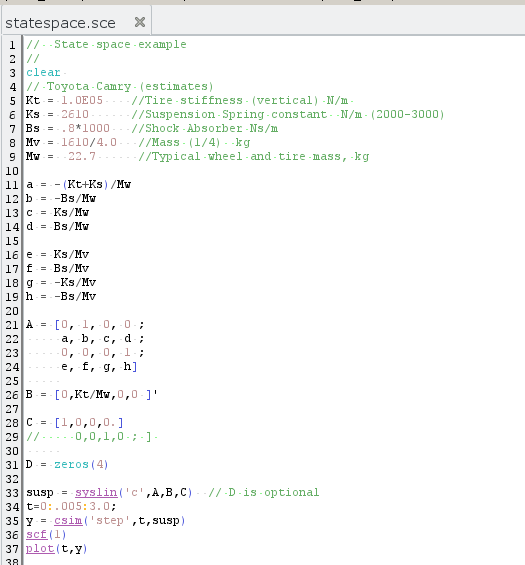
\includegraphics[width=3.5in]{figs03/ss_script.png}
\end{center}

In lines 5-9 we enter some approximate parameter values for a Toyota Camry using MKS units.  Then lines 11-19 compute the elements of $A$ based on the equations derived in the example.  Finally $A,B,C,D$ are put together in lines 21-31.   Note that for a Single-Input-Single-Output system (the only type in this course), $B$ must be a column vector, and $C$ a row vector.  

In line 33 we create a linear system object named {\tt susp} which contains the full system equations.  Finally the step response is plotted using the Scilab {\tt csim()} function 
(Figure \ref{graphsuspensionstep}).

\begin{figure}[b]\centering
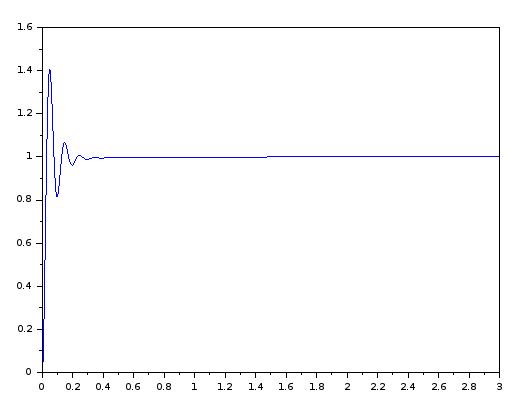
\includegraphics[width=3.5in]{figs03/ss_stepresp.png}
\caption{Step response of the car suspension system (time for new shocks!).}\label{graphsuspensionstep}
\end{figure}

Let's visualize the step response in state space instead of the time domain.   We'll choose 
a plane which is a subspace of state space: $[x_2, \dot{x}_2]$.   We add the following lines
to the script:

\begin{center}
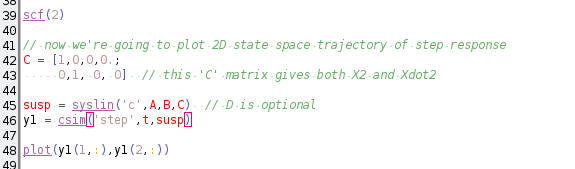
\includegraphics[width=3.5in]{figs03/ss_xyplot.png}
\end{center}

The result (Figure \ref{graphstatespacespiral}) shows the position $x_2$ on the X axis and velocity,
$\dot{x}_2$ on the y axis.  The system trajectory is a startling spiral from the inital point
($x_2=0, \quad \dot{x}_2=0$), to the final point ($x_2=1, \quad\dot{x}_2=0$).   Time is not explicitly shown but the overshoot indicates the overshoot in the step response and its convergence to the steady state 
value (1.0). 


\begin{figure}[b]\centering
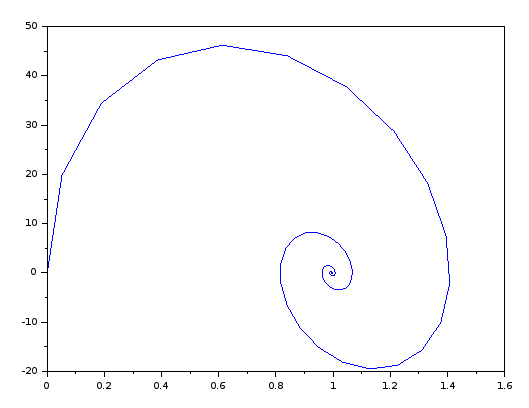
\includegraphics[width=3.5in]{figs03/ss_spiral_response.png}
\caption{Step response of the car suspension system in state space.  X axis is $x_2$ the position of the wheel, and Y axis is $\dot{x}_2$ the velocity of the wheel.}\label{graphstatespacespiral}
\end{figure}


\end{document}

